% !TEX root=/home/tavant/these/manuscript/src/manuscript.tex


\section*{Plasma models and simulations}
\label{sec-simulations}
\addcontentsline{toc}{section}{Plasma models and simulations}

Depending on the pressure, energy, and time scale, different models are more adapted to describe the plasma.
There are mainly two distinct models.
The first is the \emph{kinetic} description of the species of the plasma, via the Boltzmann equation.
The second uses a \emph{fluid} description of the species, by means of moments.
% 
% \begin{figure}[hbtp]
%   \centering
%   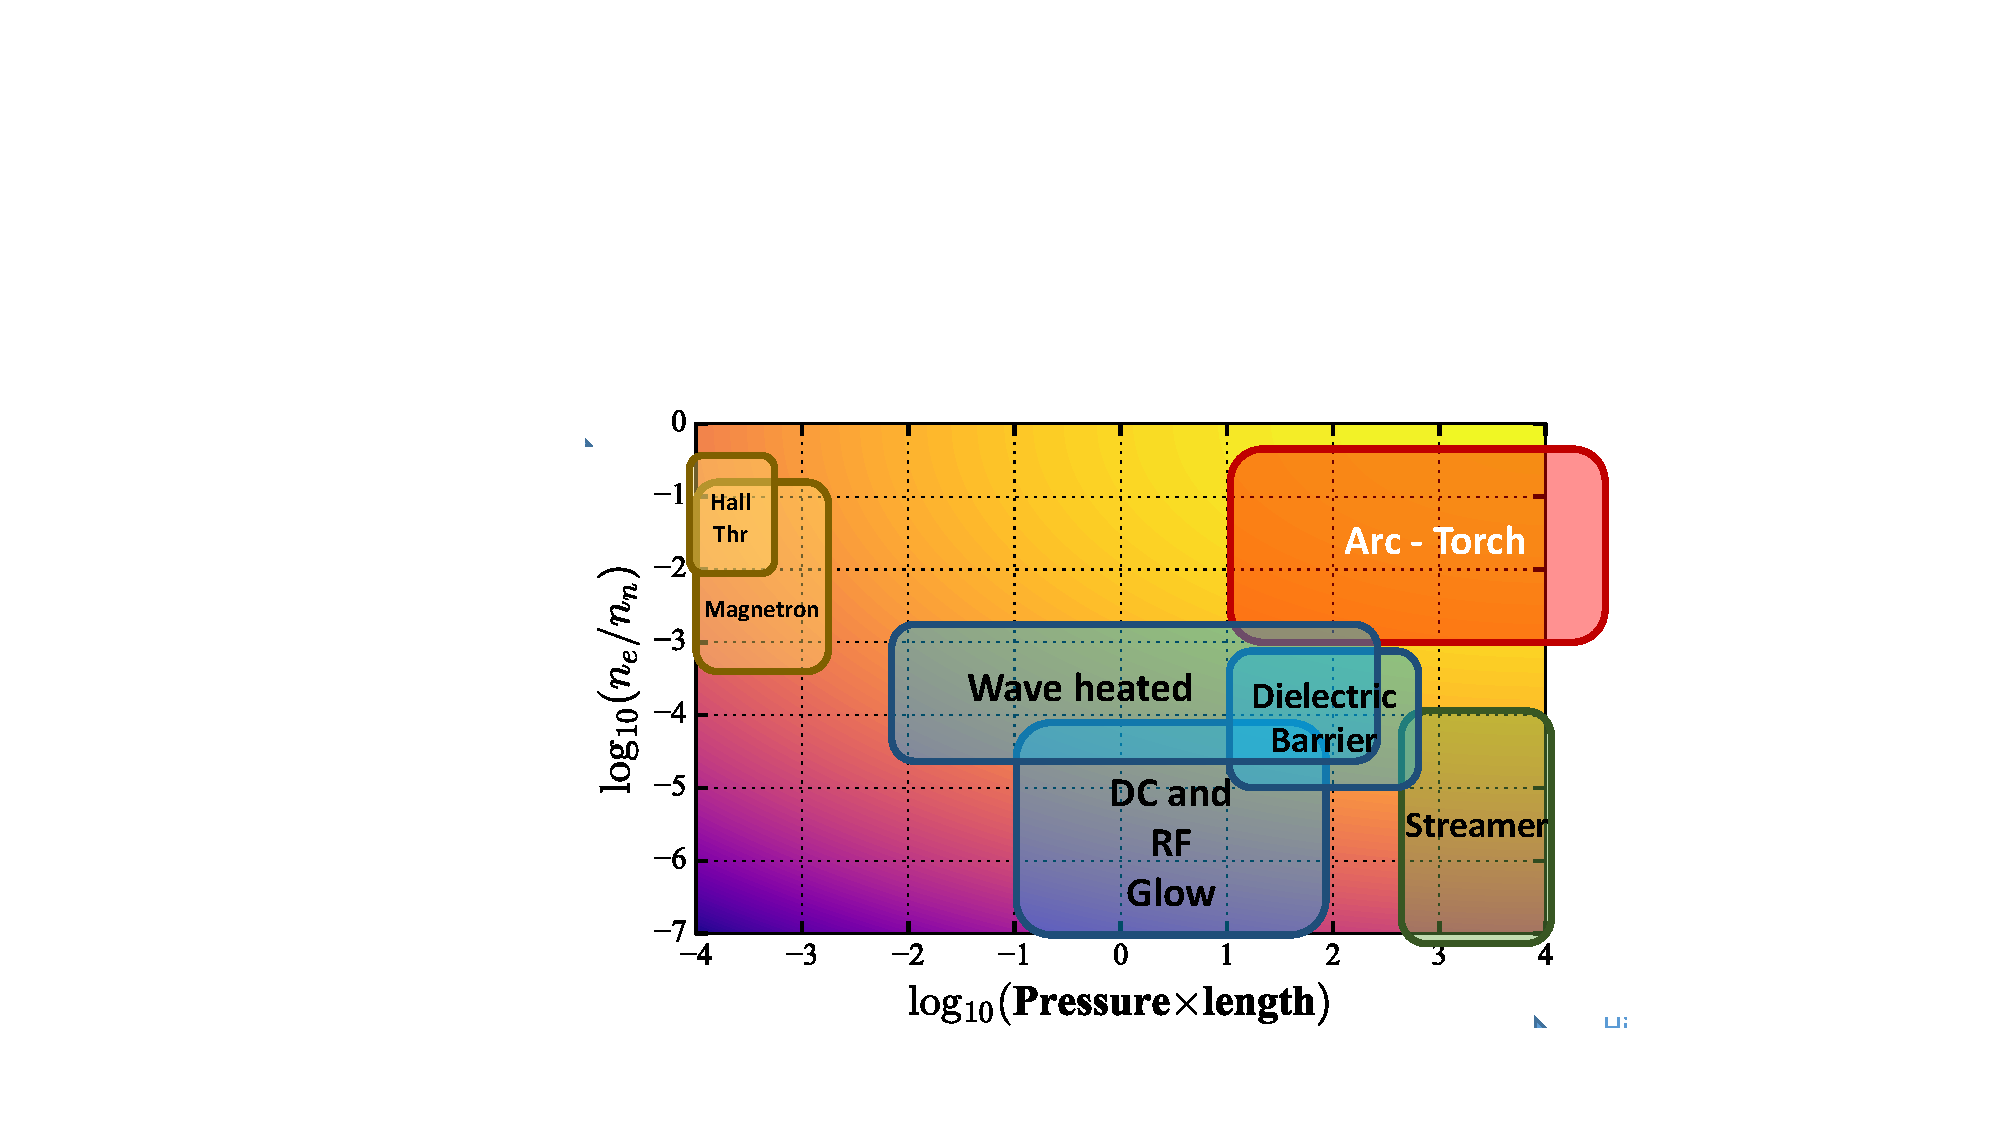
\includegraphics[width=\defaultwidth]{Chart}
%   \caption{}
%   \label{fig-chart}
% \end{figure}


\paragraph{Boltzmann equation \\}
The Boltzmann equation in \cref{eq-boltzmann} describes the evolution of the particles (atoms, ions, and electrons) in the phase space.
The phase space is the set of each possible position $\vect{x}$ and velocity $\vect{v}$ that can be attained by a particle.
The evolutions in the phase space are due to forces, diffusion, and collisions.

\begin{equation} \label{eq-boltzmann}
\deriv{f}{t}  + \vect{v} \cdot \grad_{\vect{x}} f + \vect{F} \cdot  \grad_{\vect{v}} f = \deriv{f}{t} \at{\rm coll}
\end{equation}
where $f$ is the distribution function of the particle at $\vect{x}, \vect{v}$, and $\deriv{f}{t}\mid_{\rm coll}$ denotes the effects of the collisions, $\grad$ is the gradient in both the positions (subscript $\vect{x}$) and the velocities (subscript $\vect{v}$)  and $\vect{F}$ is the force applied to the particle.
In the general electromagnetic case,
\begin{equation*} \label{eq-forceEM}
  \vect{F} =  q \vect{E} + q \vect{v} \times \vect{B}
\end{equation*}
with $q$ the particle charge, $\vect{E}$ the electric field, and $\vect{B}$ the magnetic field.

The distribution function of the stationary Boltzmann equation without collision, also known as the stationary Vlasov equation, is
\begin{equation} \label{eq-Maxwellian}
  f(\vect{v}) = N (\frac{m}{2 \pi k_B T})^{3/2} \exp \lp - \frac{q \phi + m v^2/2}{k_B T } \rp,
\end{equation}
with $k_B$ the Boltzmann constant, $T$ is the temperature of the particle population, and $\phi$ is the electric potential, defined as $\vect{E} = \grad \phi$, and $N$ is the density at the position where $\phi = 0$.
\cref{eq-Maxwellian} is the Maxwell-Boltzmann distribution function in velocity.
The unit of the temperature $T$ is the Kelvin, but in plasma physics, it is usual to us ${\rm T}$, defined as
\begin{equation} \label{eq-T_def}
  e {\rm T} = k_B T.
\end{equation}
The unit of ${\rm T}$ is therefore the Volt.
The equivalence is $1 \,\volt \simeq 10^4 \,\kelvin$.
\footnote{It is usual to find in the literature the temperature ${\rm T}$ expressed in electron-Volt eV.
This is not coherent with the definition \cref{eq-T_def}, but mark the fact that the temperature is related to an energy via $k_B$. therefore, the reader needs not to be confused by the equivalence between the electron-Volt and the Volt.  }
\nomenclature[Q]{\ensuremath{ \rm T}}{Temperature in Volt }
\nomenclature[Q]{\ensuremath{ T}}{Temperature in Kelvin }

We can write \cref{eq-Maxwellian} with the particle kinetic energy $\epsilon = \frac{1}{2} m v^2$ to defined the energy distribution function
\begin{equation} \label{eq-Maxwellina_energy}
  f_{\epsilon}(\epsilon) = N \frac{2 \sqrt{\epsilon}}{{k_B T}^{3/2} \sqrt{\pi}} \exp \lp- \frac{q \phi + \epsilon}{k_B T} \rp.
\end{equation}
The factor $\sqrt{\epsilon}$ in \cref{eq-Maxwellina_energy} appears because of the integration of the velocity distribution function $f$ over the three direction.
Thus, it is convenient to use the energy probability function 
\begin{equation} \label{eq-EPF}
  f_P(\epsilon) = \frac{f_{\epsilon}}{\sqrt{\epsilon}}.
\end{equation}

We name the Maxwellian distribution function the distribution
\begin{equation} \label{eq-Maxwelliantwo}
  f_{\rm M}(\vect{v}) = n (\frac{m}{2 \pi k_B T})^{3/2} \exp \lp - \frac{ m v^2/2}{k_B T } \rp,
\end{equation}
with $n$ the density.
One can show that the Maxwellian distribution function is the solution of the Boltzmann with only elastic collisions \citet{lieberman2005}.
In one dimension, the Maxwellian distribution function becomes
\begin{equation}
  f_{\rm M, 1D}(v) =  n (\frac{m}{2 \pi k_B T})^{1/2} \exp \lp - \frac{ m v^2/2}{k_B T } \rp,
\end{equation}

\paragraph{Fluid equations \\}
The description on the plasma in 7 dimensions (3 of space, 3 of velocity, and one of time) can complicate the resolution of the Boltzmann equation.
If the precise description of $f$ is not needed, we can instead use the first moments of \cref{eq-boltzmann} on the velocity to obtain a set of simpler equations.

The first equation is obtained by integrating \cref{eq-boltzmann} over the velocity space, which gives
\begin{align}
    & \iiint_{\vect{v}}  \deriv{f}{t} d^3v &&+&& \iiint_{\vect{v}}  \vect{v} \cdot \grad_{\vect{x}} f  d^3v &&+&&  \iiint_{\vect{v}}  \vect{F} \cdot  \grad_{\vect{v}} f  d^3v && = && \iiint_{\vect{v}}  \deriv{f}{t} \at{\rm coll} \nonumber  \\ 
   \iff &  \deriv{n}{t} &&+&&  \grad_{\vect{x}}  \cdot  ( \vect{u} n) &&+&& 0 &&=&& S_{\rm iz}   \label{eq-conc}
\end{align} 
where $n=\iiint f d^3v$ is the density, $\vect{u} = \frac{1}{n} \iiint \vect{v} f d^3v$ is the mean velocity, and $S_{\rm iz}$ is the source term of particle due to ionization.
\Cref{eq-conc} is the continuity equation for a given species.
In a similar fashion, integrating the Boltzmann equation times the velocity and the kinetic energy gives the momentum conservation equation and the energy conservation equation, respectively.
This set of equations is simpler, although it relies on additional hypotheses.

One of them is the closure of the system.
Indeed, the continuity equation describes the evolution of the density $n$ but needs the mean velocity $\vect{u}$.
However, the velocity is described by the momentum conservation equation that needs the temperature $T$, and so on.
To close the system, one has to make a hypothesis on the higher moment of the distribution function.
A usual closure is the isothermal hypothesis, that fixes the temperature. 
Hence, the energy conservation equation is not needed.
Other possible closures are the adiabatic hypothesis (no heat flux, the \nth{3} moment of $f$), the polytropic law linking the evolution of $n$ with $T$, or the Fourier law for heat diffusion.
% \inlinenote{Should we write the closes as equations ? $q = 0$, $T_e n_e ^{a}=cst$, etc. ?}

Besides, one may be led to believe that the temperature is defined by the Maxwell-Boltzmann distribution \cref{eq-Maxwellian}, and therefore that the fluid set of equation equations need to use hypothesis that $f = f_{\rm M}$.
As a matter of fact in this work, the temperature is defined by the second moment of the distribution function
\begin{equation} \label{eq-defTe}
  k_B T = \frac{m}{3 n} \iiint (\vect{v} - \vect{u})^2 f(\vect{v}) d^3v.
\end{equation}
It happens that in the case of the Maxwell-Boltzmann distribution, the quantity define by \cref{eq-defTe} is the denominator of the argument of the exponential in \cref{eq-Maxwellian}.

The integral in \cref{eq-defTe} can be decomposed over the three directions $x,y$, and $z$ as
\begin{equation} \label{eq-3Te}
  k_B T = \frac{m}{3 n} \sum_{i=x,y,z} \iiint (v_i - u_i)^2 f(\vect{v}) d^3v = \frac{ T_x + T_y + T_z}{3},
\end{equation}
which defines the directed temperatures.
A distribution is said anisotropic if the three temperatures differ.

\subsection*{Plasma simulation models} \label{subsec-simulations}
As there are two different models to describe the plasma, there are two different simulation approaches\string: the fluid simulations and the kinetic simulations.
The fluid simulations solve the moments of the distribution function (the density, mean velocity, and usually the temperature of the species), and the electromagnetic fields.
Depending on the conditions, the system of equations can be simplified before resolution.
Under the electrodynamic conditions, mainly for space plasmas and fusion, the Maxwell equations are coupled to the fluid equations leading to magnetohydrodynamics (MHD).
In the case of electrostatic conditions, as it is usual for Low-Temperature (LT) plasmas, the Poisson equation is coupled to the fluid equations.
In most of LT plasmas, the plasma in quasi-neutral except in small regions as plasma sheaths close to walls.
It is also common to neglect inertia terms and assume a steady-state in the momentum equations, leading to the drift-diffusion approximation.
The fluid equations can be solved in \ac{3D}, \ac{2D}, or \ac{1D} for space.
In a low dimension model, the effects of the missing dimensions are usually included, for instance, in the source terms as done by \citet{barral2003a}.


\vspace{1em}
However, some phenomena can only be described via the knowledge of the distribution function.
An example of such phenomena is the particle-wave interaction, such as the Landau Damping \citep{landau1945,malmberg1964}, or the plasma-beam instability \citep{filippychev1990}, for which the gradient of the distribution function in the velocity space is important.
In contrast to the fluid descriptions, \emph{kinetic} simulations solve the distribution function $f$ for both position and velocities.
Two approaches are usually used for kinetic simulations\string:
\begin{itemize}
  \item The \ac{DK} model, that discretizes \cref{eq-boltzmann} in the full phase space.
  \item The \ac{PIC} model, which uses an ensemble of particles to discretize the distribution function.
\end{itemize} 
While the \ac{DK} simulations use a Eulerian description of the distribution function, we can see the \ac{PIC} simulations as a Lagrangian approach.
The \ac{DK} simulations can theoretically better describe the plasma, mostly because there is less numerical noise and we can model binary collisions more easily, especially Coulomb collisions.
On the other hand, \ac{PIC} simulations are much simpler to develop on both a mathematical and a computation perspective.
For instance, the kinetic effects of electron emission have been recently studied using \ac{DK} simulation by \citet{cagas2019}, while it has been done since the last century in \ac{PIC} simulations \citep{boswell1988}.


